
\section{Modeling Instrumental MET using MET Templates}
\label{sec:templates}

\subsection{Introduction}

The premise of this data driven technique is that MET in \Z plus jets events
is produced by the hadronic recoil system and {\it not} by the leptons making up the \Z.
Therefore, the basic idea of the MET template method is to measure the MET distribution in 
a control sample which has no true MET and the same general attributes regarding
fake MET as in \Z plus jets events.
%need qcd on equal footing
The original implementation of the template method used QCD dijet and multijet events
to model the instrumental MET in lepton plus jets events.
In this note, we use seperately templates derived from QCD events and photon plus
jets events. We therefore have two independent control samples which each provide
a separate prediction for the MET in the \Z plus jets sample. This gives us extra
confidence that the method is not very sensitive to the composition of the control
sample.

%need qcd on equal footing
In selecting both QCD and photon plus jets events, 
the jet selection from section \ref{sec:jetsel} is used.
%In our case, we choose a photon-like sample. 
For selection photon-like objects, the very loose photon selection described in section
\ref{sec:phosel} is used.
It is not essential for the photon sample to have high purity.
%These are not necessarily photons, but 
For our purposes, selecting jets with predominantly 
electromagnetic energy deposition in a good fiducial volume suffices to ensure that 
they are well measured and do not contribute to fake MET.

%postpone the discussion of balancing until we talk about the qcd balancing correction
%Both the control sample and the \Z plus jets background
%consist of a well measured object (either a photon or a leptonically decaying \Z) which recoils 
%against a system of hadronic jets. 
The MET in these events is dominated by mismeasurements of the hadronic system. 
To account for kinematic differences between the hadronic systems in the control vs. signal 
samples, we measure the MET distributions in the control sample in bins of the number of jets 
and the scalar sum of jet \pt. 
The Njet binning used is 2 jets and $\ge$ 3 jets. 
The sum jet \pt binning is defined by the boundaries {60, 90, 120, 150, 250, 5000}~GeV.
These MET distributions normalized to unity form the MET templates.

The prediction of the MET in each \Z event is the template which corresponds to the njet and 
sum jet \pt in the \Z event. The prediction for the \Z sample is simply the sum of all such templates.

In both the case of QCD and photon templates, a variety of triggers with different \pt thresholds 
are need in order to properly sample the templates. Each of these triggers has a different prescale
which varies over the course of data taking. It is therefore necessary to take this prescale into
account when creating the templates so that the prediciton is not biased by the lower prescale 
triggers. This is done by applying a weight to the event when filling the templates. The weight 
is the product of L1 and HLT prescales. Each trigger used has a separate set of templates, which 
in effect means that the triggers are MET distributions binned in three dimensions: njet, 
sum jet \pt, and trigger.

In order to avoid contamination of events with real MET from W bosons, events with leptons 
are vetoed when making templates.

While there is in principle a small contribution from \ttbar in the \Z sample from 
which we predict the MET distribution, it is only $\approx$2.6\% of the total sample used
(MC expectation),
as shown in table \ref{preselyieldtable}, and the data driven prediction (see Fig. 
\ref{fig:pfmet_eemm}) estimates that the \ttbar contribution to the loose signal 
region is $\approx$0.3\% of the total \Z yield. As the MET measurement in these events 
does not enter the MET prediction, this small non-\Z contribution is negligible.

The above outlines the template method and was general to both QCD and photon samples. In the 
sub-sections below, we discuss the slightly different procedure which is necessary in deriving 
and applying the two sets of templates, and then compare the results obtained from each.


\subsection{QCD Templates}
\label{sec:templatesqcd}

The QCD sample is selected using single jet triggers which are listed in appendix \ref{app:jettrig}. 
The lead jet \pt in the QCD event determines which of the trigger bins the event enters according 
to the thresholds lised in appendix \ref{app:jettrig}. In order to make a reliable prediction, 
the same quantity with the same thresholds must be used to pick template is used to predict 
a \Z event. Therefore the lead jet \pt in the \Z sample is used to pick the QCD template trigger bin.

The one significant difference between QCD and photon plus jets events is that in photon plus
jets events, the jet system may recoil against the photon. Since the photon in general 
contributes less MET to the event than the jets, the recoil against the photon tends to increase 
the MET in photon plus jets events compared to QCD events with similar njet and sum jet pt.

To model this effect, a smearing procedure is applied to the QCD templates when making the 
prediction for the \Z sample which depends on the \pt of the \Z. We estimate the magnitude 
of this effect using the photon sample by plotting the dot product of the photon \pt and the MET 
divided by the photon \pt squared:

\begin{equation}
\frac{\overrightarrow{p_T}_{photon} \cdot \overrightarrow{MET}}{|\overrightarrow{p_T}_{photon}|^2}
\end{equation}

%Victor's schmear procedure:
%
%take 0.6*zpt as z-met, assume it's in the x-direction
%for each bin,
% in 20 directions,
%  add z-met to the met in this bin in the direction of this iteration, which is 'new-met'
%  fill new template with new-met

The distribution of this quantity is peaked at 6\% and is gaussian. It does not depend strongly on 
the number of jets nor the photon \pt. We therefore take 6\% of the \Z \pt when making this 
correction as the MET contribution from the boson recoil. Then for each bin in the template, this 
MET contributin is added and averaged over a number of different angles to obtain a new template 
which is used to make the final predicition from the QCD sample.


\subsection{Photon Templates}
\label{sec:templatespho}

The photon sample used to create the photon templates is obtained from the single photon triggers 
listed in appendix \ref{app:photrig}. As in the QCD case, each trigger feeds its own set of templates 
(MET distributions binned in njet and sum jet pt).
%In order to track conditions which change over the course of data-taking
%(most notably the increased pile-up) and to increase the statistics at large photon \pt, we
%use templates obtained from multiple photon triggers ``stitched'' together. 
Each photon event enters the template for the
highest \pt photon trigger which fired in the event. 
%The resulting MET distributions in each bin of njets, sumjetpt and photon trigger are then 
%normalized to unit area, yielding an array of MET templates. 

In order to make the prediction of the MET in the \Z sample, each \Z event is assigned one unit 
area template based on its number of jets, the scalar sum of jet \pt and the \Z \pt. 
The \Z \pt enters only in choosing which bin of photon trigger to use. 
This is done because the \Z \pt is the analogous variable in the \Z sample 
to the photon \pt. The \Z \pt ranges used for each trigger are shown in appendix \ref{app:photrig}
and are chosen to take into account the turn-on of the photon trigger.

%In order to account for the different prescales of the different photon triggers (which 
%change during running), 
%each template is filled with a weight equal to the prescale of the corresponding trigger.
%After this procedure, the templates are normalized to unity.

%trig weighting move above
%If this is not done, the relative contribution of different parts of the photon
%\pt specturm will not be sampled properly. In other words, this procedure corrects and 
%smoothes the photon \pt distribution.% so that it matches the \Z \pt distribution.
%The ranges of \Z \pt chosen for each photon trigger 
%take into account the turn-on of the photon trigger and are shown below.

%old
%{\bf Claudio: currently the Z pt is used to determine which trigger template set to use. You argued earlier that instead
%\bf we should use the pt of the hadronic recoil. I have verified that this makes a negligible difference, but if you prefer,
%\bf I can switch to using hadronic recoil pt.} 

%Below was commented out, but since I notice this procedure has a large effect due to the large prescale, I think it's important to include this text.

%In order to select a photon sample whose \pt distribution matches the distribution of \Z \pt
% in our preselection, a combination of photon triggers is used.
% must be used (see below). 
%In order to account for varying prescales of the triggers in different runs,
% separate templates are created for each trigger line. 
%Each event enters the template for the highest \pt trigger which fires in the event,
% and the template is filled with a weight equal to the prescale of the corresponding trigger.
%After this procedure, the templates are normalized to unity.

%The sum of the templates for all selected \Z events then forms the 
%prediction of the MET distribution for the \Z sample. Integrating this prediction for our 
%signal regions  thus provides a data driven prediction for the \Z plus jets yields in the 
%signal regions. 
%The prediction is then formed by selecting the photon trigger based on the \pt of the \Z in the event which is being predicted

We show all the templates used in appendix~\ref{sec:appendix_templates}.

%The photon triggers, and the ranges of \Z \pt for which they are selected, are (where the ``\verb=v*='' stands for a verion number which increments with trigger menu changes):
%
%\begin{itemize}
%\item \verb=HLT_Photon20_CaloIdVL_IsoL_v*= (\Z \pt $<$ 33~GeV)
%\item \verb=HLT_Photon30_CaloIdVL_IsoL_v*= (33 GeV $<$ \Z \pt $<$ 55~GeV)
%\item \verb=HLT_Photon50_CaloIdVL_IsoL_v*= (55 GeV $<$ \Z \pt $<$ 81~GeV)
%\item \verb=HLT_Photon75_CaloIdVL_IsoL_v*= (\Z \pt $>$ 81~GeV)
%\end{itemize}
%
%The HLT requirements (as described in \cite{ref:eghlt}) on the above triggers are listed in appendix~\ref{app:photrig}.

%\begin{itemize}
%\item CaloIdVL: \\
%  H/E $<$ 0.15 (0.1), $\sigma_{i\eta i\eta} <$ 0.024 (0.04) in barrel (endcap)
%\item IsoL: \\
%  Ecal ET $<$ 5.5 + 0.012*ET, %\\
%  Hcal ET $<$ 3.5 + 0.005*ET, %\\
%  Trk PT $<$ 3.5 + 0.002*ET 
%\end{itemize}

%last year for the thresholds we used trigger value +2. This year I observe a bit slower turn-on:

%  //notes on turn on curves from drawing photon pts from data babies
%  //the 20 trig is nearly fully efficient at 21, but use 22 to be conservative
%  //the 30 trig is nearly fully efficient at 32, but use 33 to be conservative
%  //the 50 trig is nearly fully efficient at 54, but use 55 to be conservative
%  //the 75 trig is nearly fully efficient at 80, but use 81 to be conservative


\subsection{Comparison of QCD and Photon Template Predictions}
\label{sec:tempcompresults}

The procedure and templates described above are applied to the \Z sample passing the preselection 
described in section \ref{sec:yields}. In this section we do not show the \Z data but instead 
focus on the two independent data driven predictions. The results including the \Z data are given 
in section \ref{sec:results}.

Figure \ref{fig:comptemp} shows the two resulting MET predictions as well as their integrals.

The two predictions are found to be consistent with one another within their statistical and 
systematic uncertainties (systematic uncertainties on the template method are discussed in 
section \ref{sec:systematicstemp}). Therefore we see no need to derive two separate predictions 
and limits, so we choose to use the photon templates for the remainder of the note.
%because the photon plus jet event topology is 
%more similar to the \Z plus jets event topology.

\begin{figure}[hbt]
  \begin{center}
    \resizebox{0.8\linewidth}{!}{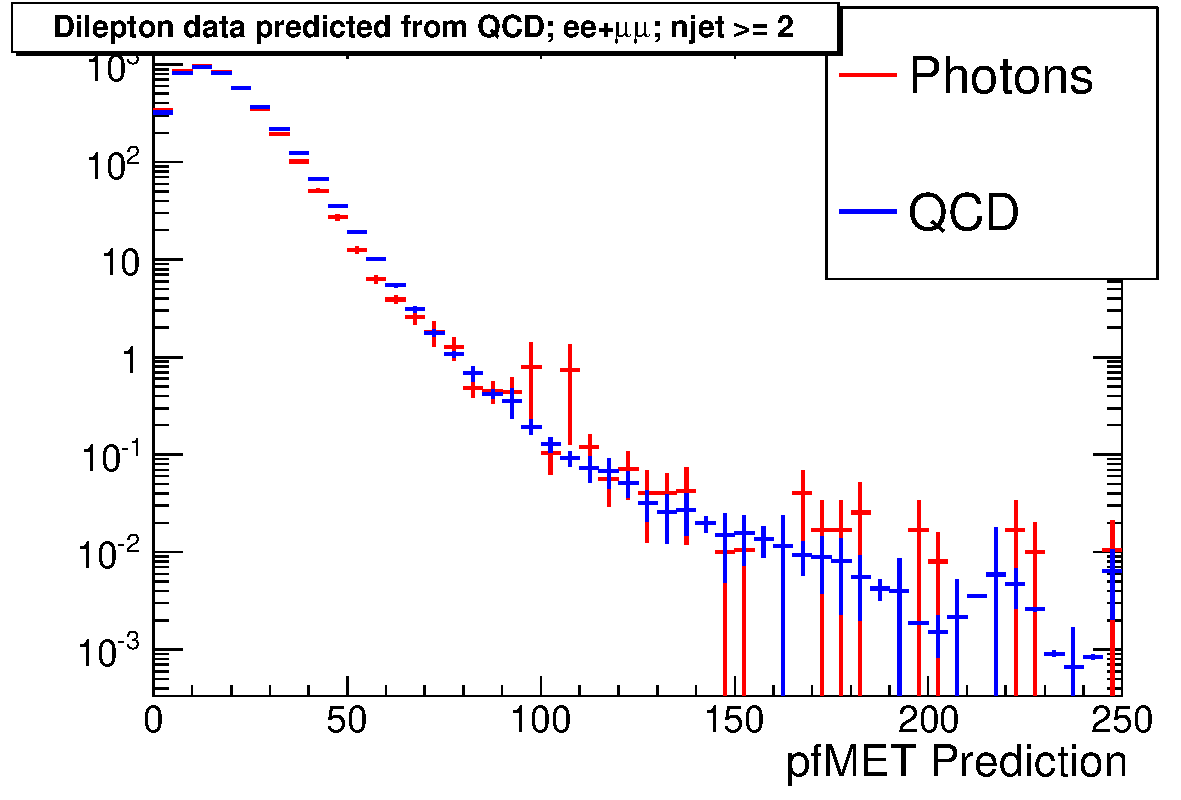
\includegraphics{plots/phoqcd_predcomp_all_nodata.pdf}}
	\\ \medskip
    %\resizebox{\linewidth}{!}{
    \begin{tabular}{r|r|r|r|r}
      MET    & $>$ 30 GeV       & $>$ 60 GeV        & $>$ 100 GeV       & $>$ 200  \\ \hline

	  photon & 406.20 $\pm$   7.10 &  13.13 $\pm$   1.23 &   1.40 $\pm$   0.62 &   0.05 $\pm$   0.02 \\
	  QCD    & 486.71 $\pm$   4.88 &  13.66 $\pm$   0.42 &   0.64 $\pm$   0.06 &   0.03 $\pm$   0.01 \\

    \end{tabular}
	%}
	\\ \medskip
    \caption{The predicted MET distribution from QCD templates (blue) and photon plus jets
	  templates (red). %(The Z data passing the preselection is used to make the prediciton 
	  %but not shown here.) %no need to restate
	  Below the plot is tabulated the integral of each prediction for
	  MET $>$ 30 GeV, $>$ 60 GeV, $>$ 100 GeV, and $>$ 200 GeV. 
	}
    \label{fig:comptemp}
  \end{center}
\end{figure}
